\documentclass[12pt]{article}
\usepackage{amsmath}
\usepackage{graphicx}
\usepackage{hyperref}
\usepackage{svg}
\usepackage[latin1]{inputenc}
\usepackage{graphicx}
\usepackage{listings}
\usepackage{hyperref}
\title{Cavendish Experiment}
\author{Murat Can Gokceaslan \\ 2013203051\\Partner:Bilal Samil Okan}
\date{01/03/19}

\begin{document}
\maketitle

\section{Abstract}
Aim of the experiment in the Cavendish's side is to find the density of the earth but for us it is to find the Gravitational Constant(G) with precision. We used a small torsion balance and it has a laser on it. So we can predict better results than historical experiment which has big masses and big torsion balance. So we determined the gravitational constant with precision.
\section{Theoretical Motivation}
\subsection{Theoretical background used in the experiment}
\subsubsection{Historical Methods}
[1] The Cavendish experiment, made in 1797/1798 by the scientist Henry Cavendish in England, was the first trial to measure the force of gravity between masses in the laboratory and the first to yield accurate values for the gravitational constant. Because of the unit conventions then in use, the gravitational constant does not appear explicitly in Cavendish's experiment. [2] Instead, the result was originally expressed as the specific gravity of the Earth or equivalently the mass of the Earth. His experiment gave the first accurate values for these geophysical constants.
\begin{center}
\includegraphics[width=0.8\textwidth]{historical.png}
[3]
\end{center}
\subsubsection{Geometry of the system}
The apparatus is used in the experiment is a torsion balance horizentally suspended from the wire with diameter lead spheres one attached to each end. Bigger balls located near the small balls and held in a place with seperate suspension system. The experiment is measuring the gravitational force between small and large masses.
\subsubsection{Equations used and their derivations}
\begin{center}
 $\tau = F * d$
 \par

 $ F = \frac{G * M * m}{r^2}$
 \par
 $\frac{2 * G * M * m}{r^2} = k * \theta_{eq}$
 \par
 $d =\frac{l_{beam}}{2}$
 \par
 F: gravitational force between the adjacent small
and large masses
\par
d: distance from the center of a small ball to the
axis of rotation
\par
G: Universal Gravitational Constant
\par
M: big mass
\par
m: small mass
\par
r: distance between small and big masses
\par
I: moment of inertia of the dumbbell system
\par
$\tau_{g}$: torque gravity
\par
$\tau_{t}$: torque tension
\par
$\kappa$: torsion constant of the fiber used
\par
$\tau$ : torque exerted by the spring
\par
$\theta$: angle of twist from its equilibrium position
\par
b: damping constant
\par
$\beta$: damping parameter
\par
$G_{exp}$: experimental value of gravitational constant
\par
$G_{nom}$: experimental value of gravitational constant
\par
------------------------------
\par
$\tau_{g} = I * \alpha = I * \ddot{\theta} = I * \frac{d^{2}\theta}{d^{2}t}$
\par
-------------------------------------
\par
Because of the gravitational torque τg the small
masses will try to turn towards to the heavier masses,
but fiber they attached will resist on motion and it
will create torque τt. This is a torsion balance. Two
opposing torques are τg and τt. Hooke’s law for torsion balance;
\par
-------------------------------------------------------
\par
$\tau = - \kappa * \theta $
\par
-------------------------------------------------------
\par
We define equilibrium angle θeq as the angle at which
there is no torque τ = 0 due to the torsion of the
fiber.We convert voltage data to angle θ by using conversion factor.
\par
-------------------------------------------------------
\par
\includegraphics[width=0.5\textwidth]{torsion_balance}
\par
$\Delta \theta = 2 \alpha$
\par
$dl = \frac{\Delta S_{mean}}{2}$
\par
$\Delta \theta = tan^{-1}(\frac{dl}{L})$
\par
Conversion factor:
$\alpha = \frac{\Delta \theta}{\Delta V}$
\par
$V_{eq} = \frac{V_{damped} - V_{mean}}{2}$
\par
$\theta_{eq} = V_{eq} * \frac{\Delta \theta}{\Delta V}$
\par
----------------------------------------------------
\par
If it is an ideal system, it does a harmonic oscillation
\par
----------------------------------------------------
\par
$I = \ddot{\theta} = - \kappa \theta$
\par
$I = \ddot{\theta} + \kappa * \theta = 0$
\par
The solution is:
\par
$\theta = A sin(w_{0} t)$
\par
$\omega_{0} = \sqrt{\frac{\kappa}{I}}$
\par
--------------------------------------------------
\par
However, our system has friction, so this motion will
fade away by getting smaller each period of motion.
The reason of damping in an oscillating system is friction. Differential equation for underdamped motion;
\par
--------------------------------------------------
\par
$I \ddot{\theta} + 2 b \dot{\theta} + \kappa \theta =0 $
\par
--------------------------------------------------
\par
So the solution is :
\par
$\theta = A e^{- \beta t} sin(\omega_{d}t + \phi) + C_{1}$
\par
--------------------------------------------------
\par
$\beta = \frac{b}{2I}$
\par
--------------------------------------------------
\par
We stop changing the position of the masses and observe the damping case. Energy and the amplitude of
the sinusoidal wave start to decrease.
\par
--------------------------------------------------
\par
$\omega_{d} = \sqrt{\omega_{0}^2 - \beta^{2}}$
\par
--------------------------------------------------
\par
$\kappa = \omega_{0}^2 I$
\par
--------------------------------------------------
\par
$\frac{\kappa \theta_{eq}}{2 d} = \frac{G * M * m}{r^{2}}$
\par
--------------------------------------------------
\par
$G = \frac{\kappa \theta_{\theta} r^{2}}{2 M m d}$
\par
--------------------------------------------------
\par
$Err = \frac{|G_{nom} - G_{exp}}{2} $
\par
\end{center}
\section{Experiment}
\subsection{Setup and Apparatus}
\includegraphics[width=1\textwidth]{experiment}
\subsubsection{Laser}
Laser is used to point out the position of small masses
\subsubsection{Scale}
Laser is dropping on the ruler scale so that we can determine the position changed in on period
\subsubsection{Torsion balance with large masses}
This is the most important thing in the experiment. We use large masses to create a gravitational attraction between small & large masses. So that this creates a oscillation over the torsion and masses.
\subsubsection{Standar Ruler}
Ruler can measure data in 2 meters with 0.01 cm standard deviation.
\subsubsection{Data Getter}
We use computer as data getter so it gives us V/s graph.
\subsection{Procedure}
1) We first measure the distance between scale and the mirror inside of torsion balance.
\par
2) Then we observe if laser is dropping down on the scale.
\par
3) If it is dropping on the scale then we check the computer that the torsion balance system has small osciallation using the computer
\par
4) We start moving the scale opposite sides till the system gets resonance. (Firstly it will increase the amplitude of the graph then it will stop increasing and this is the point where you understand that it is a resonance point)
\par
5) After taking a 5 data on resonance we stop changing position of scale and observe the damped oscillation. (We observed the damped oscillation with reverse side)
\par
\subsection{Data}
\subsubsection{S Values}
\begin{center}
\begin{tabular}{ c c c c }
 Smax(cm) & Smin(cm) & $\Delta S$ & $\simga S$ &
 +1.7 & -1.6 & 3.3 & 0.08 &
 +1.8 & -1.5 & 3.3 & 0.08 & 
 +1.8 & -1.8 & 3.6 & 0.08 &
 +1.8 & -1.7 & 3.5 & 0.08 &
 +1.9 & -1.8 & 3.7 & 0.08 &
\end{tabular}
\par
This is the max and min points on scale in resonance
\par
\end{center}
\subsubsection{Constants}
\begin{center}
\begin{tabular}{ c c c c}
$Constants$&Values&Error&Unit&
 $M_{1}$&1.0385&0.001&kg&
 $M_{2}$&1.0386&0.001&kg&
 $m_{1}$&0.014573&0.000001&kg&
 $m_{2}$&0.014545&0.000001&kg&
 $M_{avarage}$&1.0385&0.001&kg&
 $m_{avarage}$&0.014559&0.000001&kg&
 DM&0.146766&0.000066&m&
 $ds_{1}$&0.013452&0.000048&m&
 $ds_{2}$&0.013468&0.000048&m&
 $d$&0.066653&3.71E-05&m&
 $D_{L1}$&0.05612&0.00009&m&
 $D_{L2}$&0.05629&0.00017&m&
 W&0.0351&0.0001&m&
 $G_{1}$&0.0007&0.0002&m&
 $G_{2}$&0.0002&0.0002&m&
 r&0.0461025&0.000158&m&
 $f_{d}$&0.0349162&0.000321&m&
\end{tabular}
\end{center}
\section{Analysis}
\subsection{How did I make the analysis}
1) I calculated the $w_{d}$ (Damping Frequency) and $\beta$ (Damping constant) by getting the points from data so the $w_{d} = \frac{2\pi}{T}$. Where T is the period of damped oscillation. So $\omega_{d} = 0.288$ rad/s .
\par
2) I calculated the $\beta$ using the equation $ \beta = \dfrac{\ln(\frac{V_{1}}{V_{2}})}{t_{2}-t_{1}}$ and $\beta = \dfrac{\ln(\frac{0.392}{0.349})}{217.9}$ so $\beta = 0.0005 rad/s$ also
$\beta = \dfrac{\ln(\frac{0.349}{0.321})}{230}$ so $\beta = 0.00069 rad/s$
So the $w_{d(average)} = 0.000595 rad/s$ 
and  $\sigma_{w_{d}} = 0.0001343$
\par
3) So the $\kappa = 1.90688 * 10^{-9} N.m / rad$
\par
4) Moment of Inertia: $I = 0.0001 ± 0.0879x10−5 $
\par
5) $\Delta V = 0.32778$ & $\sigma_{\Delta V} = 0.00336$
\par
6) Calculation of $\theta_{eq}$
\par
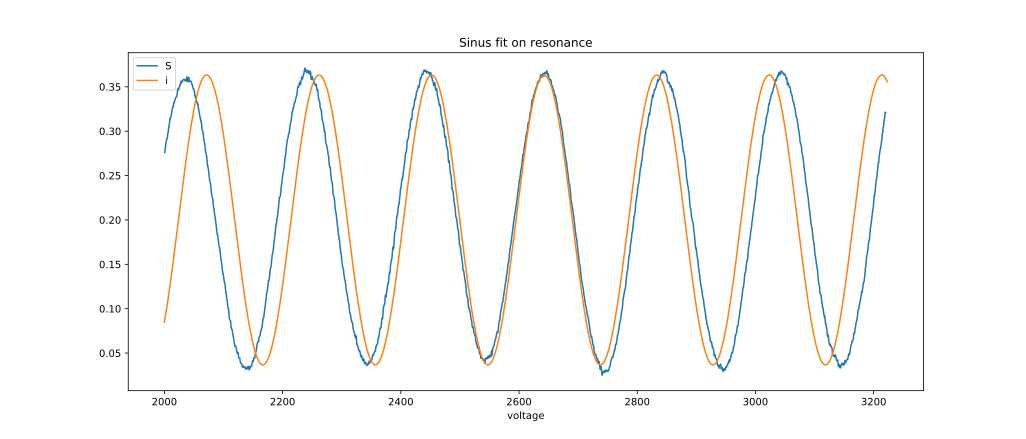
\includegraphics[width=0.8\textwidth]{sine_fit.png}
\par
7) $\Delta S_{mean} = 3.48$ and $  \sigma_{\Delta S} = 0.08$
\par
8) $\alpha = \frac{\Delta V }{\Delta \theta} = 0.3356$ and $\sigma_{\alpha} = 0.005873$
\par
9)From these results $\Delta \theta_{eq} =  0.11 rad$ and $\sigma_{\Delta \theta} = 0.0005 rad$
\par
10) so the $G = 2.9746 * 10^{-11}$ and the standard deviation of it $\sigma_{G} = 0.521 * 10^{-11}$
\section{Conclusion}
The last result is $G = 2.9746 * 10^{-11}$ and $\sigma_{G} = 0.521 * 10^{-11}$ So the therotical value $6.674 08 x 10^{-11}$ . So the therotical value is in 6 $\sigma$ away from our calculation. Posssible errors could be the glass shake changed our resonance and damped value. In addition to this, our masses affects the system. So when I go near to change the position of scale so it will create a gravitational change over small masses so that our data gets wrong.
Gravitational constant (G) has higher relative uncertainty when compared to the other fundamental
constants. Because it’s the weakest force, so it’s really difficult to calculate the pricise value of G.
\section{References}
\par
[1] \hyperref[Wikipedia]{https://en.wikipedia.org/wiki/Cavendish_experiment}
\par
[2] \hyperref[Britannica]{https://www.britannica.com/science/Cavendish-experiment}
\par
[3] \hyperref[Decoded Science]{https://www.decodedscience.org/the-cavendish-experiment-to-measure-the-gravitational-constant-g/22608/2}
\par
\section{Code and Data}
\subsection{Damped Code}
\begin{lstlisting}
import numpy as np
import matplotlib.pyplot as plt
import pandas as pd
import statistics as st
data = pd.read_csv('damped.txt', sep=" ", header=None,delimiter="\t")
datapointx = []
datapointy = []
countAll = 0
for a in range(data[1].size):
    if a > 3000:
        datapointx.append(data[0][a])
        datapointy.append(data[1][a])
        countAll += data[1][a]
mean = countAll / (data[1].size - 3000)
standard_deviation = st.stdev(datapointy)
plt.plot(datapointx, datapointy)
plt.legend("Damped")
plt.xlabel("time")
plt.ylabel("voltage")
plt.legend("Sine")
plt.show()
\end{lstlisting}
\subsection{Resonance Code, It also does the sinfit}
\begin{lstlisting}
import numpy as np
import matplotlib.pyplot as plt
import pandas as pd
import statistics as st
data = pd.read_csv('damped.txt', sep=" ", header=None,delimiter="\t")
datapointx = []
datapointy = []
countAll = 0
for a in range(data[1].size):
    if a > 4000:
        datapointx.append(data[0][a])
        datapointy.append(data[1][a])
        countAll += data[1][a]
mean = countAll / (data[1].size - 4000)
standard_deviation = st.stdev(datapointy)
plt.plot(datapointx, datapointy)
plt.legend("Resonance")
def fitterSine(t):
    w=0.03300
    A=((0.6566 - 0.33)/2)
    theta= w*t
    sin = A * np.sin(theta-60.5)
    return sin 
fity = []
timer = []
for i in range(2000,3224):
    timer.append(i)
    fity.append(fitterSine(i)+0.20)
plt.plot(timer,fity)
plt.title("Sinus fit on resonance")
plt.xlabel("time")
plt.ylabel("voltage")
plt.legend("Sine")
plt.show()

\end{lstlisting}
In the code I changed data's commas as dots. So it may not run with those txt file.  Here is the github url with datas and codes:
https://github.com/cangokceaslan/Cavendish-Experiment

\end{document}
